\chapter{Kinematic Modeling}
\section{Overview and Objectives}

This chapter addresses the kinematic modeling of the hand exoskeleton within the Digital Twin framework. Starting from the URDF representation introduced in Chapter 1, the objective is to construct a kinematic model that is both compatible with the tree-structured formulation required by standard robotics libraries and capable of accurately reproducing the closed-chain behavior of the physical mechanism.

The hand exoskeleton is characterized by multiple closed kinematic loops, which are essential to enforce coordinated motion among the links. However, such loops cannot be directly represented within the URDF formalism, which assumes a tree topology. As a consequence, the original mechanism is converted into an equivalent open-chain structure, and the loop-closure conditions are reintroduced at the computational level through constraint enforcement.

The resulting kinematic problem is therefore formulated as a constrained forward kinematics task, in which the configuration of the open-chain model is adjusted such that the geometric constraints corresponding to the closed loops are satisfied.

This formulation provides a flexible and numerically robust framework that integrates seamlessly with the Pinocchio\cite{carpentier2019pinocchio} library and serves as the foundation for the reduced-order dynamic modeling presented in the following chapter.


%%%%%%%%%%%%%%%%%%%%%%%%%%%%%%%%%%%%%%%%%%%%%%%%%%%%%%%%%%%%%%%%%%%%%%%%


\section{Kinematic Constraints Formulation}

The kinematic structure of the exoskeleton includes multiple closed loops arising from the mechanical coupling between links. To enable compatibility with the URDF representation, these loops are opened at selected revolute joints, resulting in a tree-structured model augmented by additional geometric constraints.

Let  $q \in \mathbb{R}^n$ denote the vector of generalized coordinates associated with the open-chain URDF model. The original closed-chain behavior is recovered by enforcing a set of holonomic constraints of the form:

\begin{equation}
    \Phi(q) = 0
\end{equation}

where $ \Phi : \mathbb{R}^n \rightarrow \mathbb{R}^m $ represents the loop-closure constraints.

Each constraint corresponds to a pair of auxiliary reference frames introduced at the points where the kinematic chains were opened. In the physical mechanism, these frames are required to coincide in position. Accordingly, for each pair $(A_i, B_i)$, the constraint is defined as:

\begin{equation}
    \Phi_i(q) = p_{A_i}(q) - p_{B_i}(q)
\end{equation}

where $ p_{A_i}(q), p_{B_i}(q) \in \mathbb{R}^3 $ denote the positions of the frames expressed in the world coordinate system.

By stacking all constraints, the global constraint vector is obtained as:

\begin{equation}
\Phi(q) =
\begin{bmatrix}
p_{A_1}(q) - p_{B_1}(q) \
\vdots \
p_{A_k}(q) - p_{B_k}(q)
\end{bmatrix}^T
\end{equation}

The violation of the loop-closure conditions can therefore be quantified by the norm  $|\Phi(q)|$, which provides a measure of the geometric inconsistency introduced by the open-chain approximation.

It is important to note that only positional constraints are enforced. This choice is consistent with the fact that the chains are opened at revolute joints, which inherently constrain relative orientations while leaving translational consistency as the primary requirement for closure.




\begin{figure}[h]
    \centering
    \subfloat[]{%
        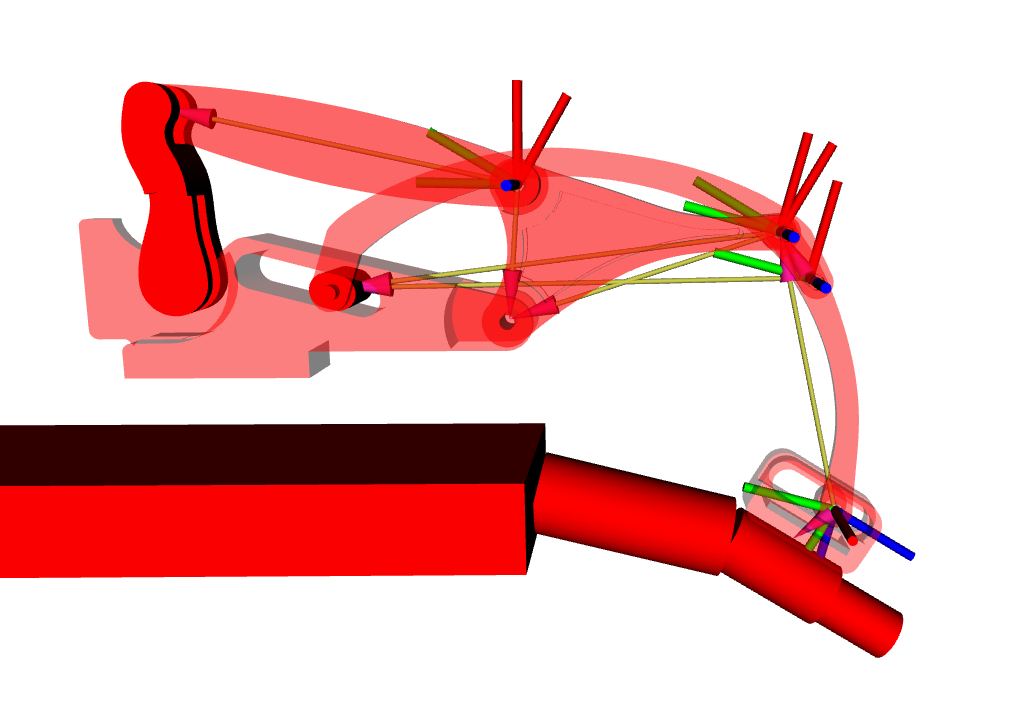
\includegraphics[scale=0.3]{images/chapter2/errori_annulati.png}
    }\\
    \subfloat[]{%
        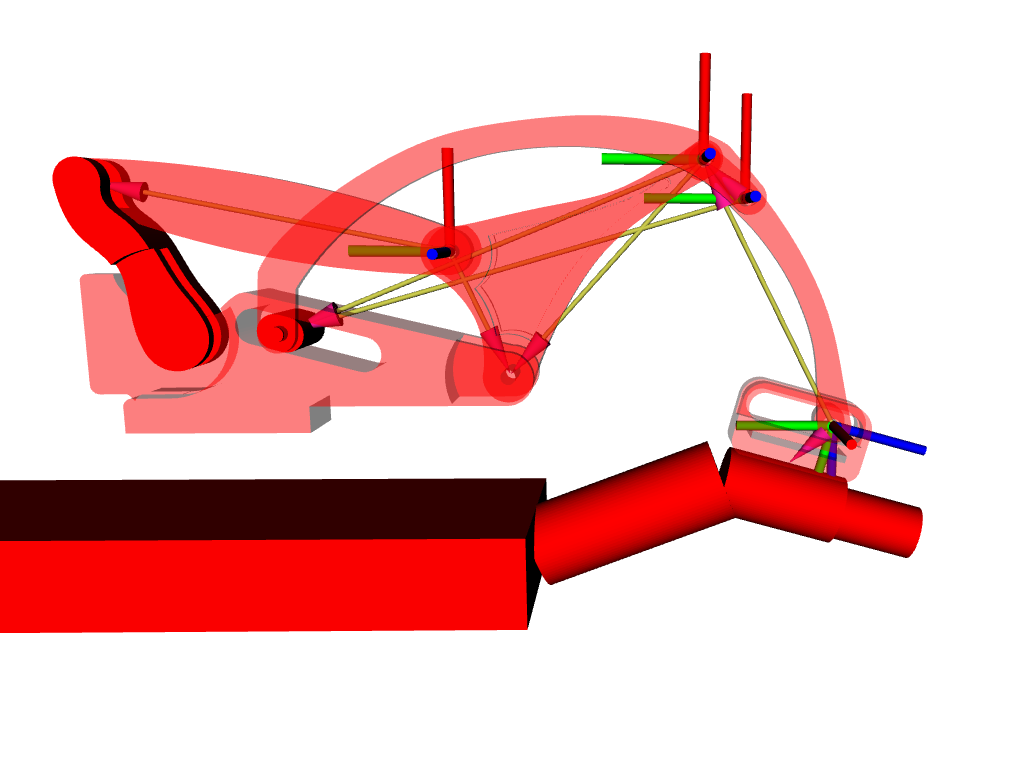
\includegraphics[scale=0.3]{images/chapter2/errori_annullati_3.png}
    }
    \caption{Auxiliary frame coincidence for the opened kinematic chain as a function of the motor joint angle.}
\end{figure}



\section{Constrained Forward Kinematics}
Given the open-chain representation and the constraint formulation introduced above, the kinematic problem is reformulated as a constrained forward kinematics task.

Let $\theta = q_{\text{crank}}$ denote the actuated joint variable. For a fixed value of $\theta$, the remaining generalized coordinates are determined by enforcing the loop-closure constraints.

To this end, a subset of generalized coordinates is selected as optimization variables. Let  $x \in \mathbb{R}^{n_r}$ denote the vector of reduced coordinates, corresponding to the joints involved in the opened kinematic chains.

The constrained forward kinematics problem is formulated as the following nonlinear least-squares optimization:

\begin{equation}
    \min_{x}  |\Phi(q(x))|^2 + \mathcal{P}(x)
\end{equation}


where:
\begin{itemize}
    \item $\Phi(q(x))$ is the constraint residual vector,
    \item $\mathcal{P}(x)$ is a penalty term introduced to regularize the solution and enforce soft bounds on selected joints.
\end{itemize}

The mapping $q(x)$ is defined by assigning the optimization variables to the corresponding joint indices while keeping the actuated joint $\theta$ fixed.

This formulation yields a configuration $q(\theta)$ that satisfies the geometric constraints and reconstructs the closed-chain kinematics of the mechanism.




\section{Numerical Solution Strategy}

The nonlinear least-squares problem is solved using a trust-region reflective algorithm, which provides robust convergence properties in the presence of bounds and nonlinearities.

At each evaluation of the residual function, the forward kinematics of the open-chain model is computed using the Pinocchio library, and the positions of the auxiliary frames are updated accordingly. The constraint residual vector is then constructed by evaluating the relative position errors between each pair of frames:

\begin{minted}{python}

    def closure_error(self, q):
    pin.forwardKinematics(self.model, self.data, q)
    pin.updateFramePlacements(self.model, self.data)

    e = []
    for ida, idb in self.frame_ids:
        e.extend(
            self.data.oMf[ida].translation -
            self.data.oMf[idb].translation
        )
    return np.array(e)

\end{minted}

The resulting vector collects all loop-closure violations and directly corresponds to the constraint function  $\Phi(q)$.

To enforce the constraints, the following residual function is minimized:

\begin{minted}{python}

    def residuals(x):
        for i, jid in enumerate(self.idx_opt):
        q[jid] = x[i]

        
        e = self.closure_error(q)

        medial = x[6]
        penalty = 0.0

        if medial < -2.0:
            penalty += (medial + 2.0)**2
        if medial > 0.0:
            penalty += (medial - 0.0)**2

        return np.hstack([e, np.sqrt(penalty)])
        
\end{minted}

The first component of the residual corresponds to the constraint violation, while the additional term acts as a soft regularization enforcing mechanically admissible configurations.

The optimization problem is solved using the following routine:

\begin{minted}{python}

    sol = least_squares(
        residuals,
        x0,
        method='trf',
        bounds=(lower, upper),
        xtol=1e-8,
        ftol=1e-8,
        gtol=1e-8
    )

\end{minted}

The solver is warm-started using the previous solution, exploiting the continuity of the motion and improving convergence speed.

The solution is accepted only if the constraint violation satisfies:

\begin{equation}
    |\Phi(q)| < \varepsilon
\end{equation}


ensuring that the reconstructed configuration is consistent with the closed-chain geometry.



\section{Discussion and Role in the Digital Twin}
The proposed kinematic formulation establishes a clear separation between the geometric representation of the mechanism and the enforcement of loop-closure constraints. This enables the use of a standard URDF-based model while preserving the physical consistency of the original closed-chain system.

A key outcome of this approach is the implicit mapping:

\begin{equation}
    q = q(\theta)
\end{equation}

which associates each value of the actuated joint with a unique configuration satisfying the constraint equations.

From an implementation standpoint, this mapping is computed numerically at runtime by solving the constrained optimization problem described above. The resulting configuration is then used as input for subsequent dynamic computations.

The numerical pipeline can be summarized as follows:

\begin{minted}{python}

    # Given theta (crank angle)
    q[idx_theta] = theta

    # Solve loop-closure constraints
    sol = least_squares(...)

    # Reconstruct full configuration
    q_consistent = q.copy()

\end{minted}

This procedure ensures that every configuration used in the Digital Twin is kinematically admissible and consistent with the original mechanism.

The mapping $q(\theta)$ plays a fundamental role in the dynamic modeling presented in Chapter 3. In particular, it defines the constraint manifold onto which the full multibody dynamics is projected, enabling the reduction of the system to a single-degree-of-freedom representation.

The kinematic solver therefore constitutes a core component of the Digital Twin architecture, bridging the gap between the URDF-based representation and the physically consistent simulation of the mechanism.
